% Created 2021-01-12 Tue 23:18
% Intended LaTeX compiler: pdflatex
\documentclass[11pt]{article}
\usepackage[utf8]{inputenc}
\usepackage[T1]{fontenc}
\usepackage{graphicx}
\usepackage{grffile}
\usepackage{longtable}
\usepackage{wrapfig}
\usepackage{rotating}
\usepackage[normalem]{ulem}
\usepackage{amsmath}
\usepackage{textcomp}
\usepackage{amssymb}
\usepackage{capt-of}
\usepackage{hyperref}
\author{Adriel Benati de Melo}
\date{12 de Janeiro}
\title{Lista de Exercícios 2}
\hypersetup{
 pdfauthor={Adriel Benati de Melo},
 pdftitle={Lista de Exercícios 2},
 pdfkeywords={},
 pdfsubject={},
 pdfcreator={Emacs 27.1 (Org mode 9.4.4)}, 
 pdflang={English}}
\begin{document}

\maketitle

\section*{4)}
\label{sec:org85f1683}

\subsection*{a) e b)}
\label{sec:org9bd919e}

Tomado o conjunto (7, 8, 6, 10, 5, 9, 4, 12, 7, 8), tem-se que:

\begin{verbatim}
conjunto <- c(7, 8, 6, 10, 5, 9, 4, 12, 7, 8)

media <- mean(conjunto)
desvp <- sd(conjunto)

cat(sprintf('Média do conjunto =  %1.0f\n', media))
cat(sprintf('Desvio padrão do conjunto = %1.0f\n', desvp))
\end{verbatim}

\begin{verbatim}
Média do conjunto =  8
Desvio padrão do conjunto = 2
\end{verbatim}

\section*{13)}
\label{sec:org9e04ff5}

\begin{verbatim}
             [,1]
Min.     1.000000
1st Qu.  2.000000
Median   4.000000
Mean     4.306977
3rd Qu.  6.000000
Max.    12.000000
\end{verbatim}

\section*{19)}
\label{sec:orgec9c189}

\subsection*{a)}
\label{sec:org4723154}

Utilizando-se do programa em R a seguir, é possível determinar o
diagrama de ramo-e-folhas.

\begin{verbatim}
dist <- c(1.8, 2.5, 0.4, 1.9, 4.4, 2.2, 3.5, 0.2, 0.9, 1.4, 1.1,
1.7, 1.2, 2.3, 1.9, 0.8, 1.5, 1.7, 1.4, 2.1, 3.2, 15.1, 2.1, 1.4,
0.5, 0.9, 1.7, 0.5, 0.8, 3.7, 1.4, 1.8, 2.0, 1.1, 1.0, 0.8)

stem(dist, scale = 2)
\end{verbatim}

\begin{verbatim}

The decimal point is at the |

 0 | 245588899
 1 | 0112444457778899
 2 | 011235
 3 | 257
 4 | 4
 5 | 
 6 | 
 7 | 
 8 | 
 9 | 
10 | 
11 | 
12 | 
13 | 
14 | 
15 | 1

\end{verbatim}

\subsection*{b)}
\label{sec:orgae22e82}

\begin{verbatim}
dist <- c(1.8, 2.5, 0.4, 1.9, 4.4, 2.2, 3.5, 0.2, 0.9, 1.4, 1.1, 1.7, 1.2, 2.3, 1.9, 0.8, 1.5, 1.7, 1.4, 2.1, 3.2, 15.1, 2.1, 1.4, 0.5, 0.9, 1.7, 0.5, 0.8, 3.7, 1.4, 1.8, 2.0, 1.1, 1.0, 0.8)

aaa <- summary(dist)

ccc <- c(0.4, 1.6, 2.8, 4.2, 8.8)
bbb <- summary(ccc)

cbind(aaa, bbb)
\end{verbatim}

\begin{verbatim}
           aaa  bbb
Min.     0.200 0.40
1st Qu.  0.975 1.60
Median   1.600 2.80
Mean     2.025 3.56
3rd Qu.  2.100 4.20
Max.    15.100 8.80
\end{verbatim}


Comparando os dados da empresa AAA e BBB, percebe-se que a empresa AAA é a que tem o os extremos mais notáveis, com um extremo superior de 15,1 comparado ao de 8,80 da empresa BBB. Exceto isso, os valores da empresa BBB são em geral mais altos que os da empresa AAA, indicando que os funcionários daquela viajam mais do que os desta.

\subsection*{c)}
\label{sec:orgd8e4dc9}

\begin{verbatim}
dist <- c(1.8, 2.5, 0.4, 1.9, 4.4, 2.2, 3.5, 0.2, 0.9, 1.4, 1.1, 1.7,
1.2, 2.3, 1.9, 0.8, 1.5, 1.7, 1.4, 2.1, 3.2, 15.1, 2.1, 1.4, 0.5, 0.9,
1.7, 0.5, 0.8, 3.7, 1.4, 1.8, 2.0, 1.1, 1.0, 0.8)

aaa <- summary(dist)

bbb <- c(0.4, 1.6, 2.8, 4.2, 8.8)

png(file = "boxplot.png")

boxplot(aaa, bbb,
		main = "Diagrama de caixas: comparação entre AAA e BBB",
		names  = c('aaa', 'bbb'))

dev.off()
\end{verbatim}

\begin{center}
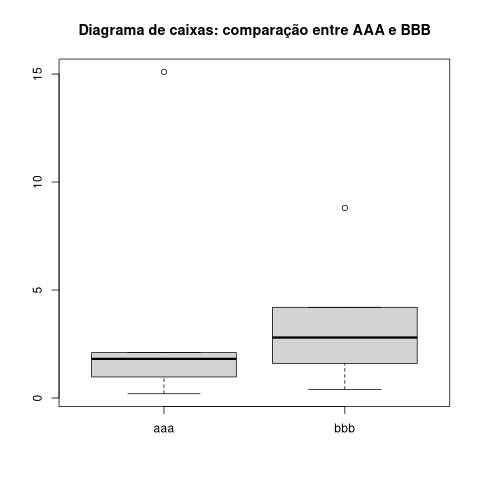
\includegraphics[width=.9\linewidth]{boxplot.png}
\end{center}
\end{document}